\documentclass[11pt,a4paper]{article}

\usepackage[margin=25mm]{geometry}
\usepackage{graphicx}
\usepackage{parskip}
\setlength{\parskip}{0.4\baselineskip}
\setlength{\parindent}{0pt}
\usepackage{caption}
\captionsetup{skip=3pt, belowskip=0pt, font=small, labelfont=bf}
\usepackage[T1]{fontenc}
\usepackage[utf8]{inputenc}
\usepackage{amsmath}
\usepackage{natbib}
\usepackage[hidelinks]{hyperref}
\usepackage{cleveref}
\usepackage{float}

\title{\vspace{-2cm}Reproducing a Tuning-Free Plug-and-Play algorithm for Sparse-View CT \\
\vspace{0.5cm}
\subtitle Executive Summary}
\author{Emilia Zabrzanska}
\date{July 2026}

\begin{document}
\maketitle

Sparse-view computed tomography (CT) reduces patient radiation dose by acquiring fewer projection angles, at the cost of creating a more ill-posed reconstruction problem. The Tuning-Free Plug-and-Play (TFPnP) method of~\citet{Wei2022TFPnP} addresses this by using reinforcement learning (RL) to select the ADMM hyperparameters automatically. This project reproduces TFPnP from scratch within the LION toolbox~\citep{Biguri2024LION} for 30-view parallel-beam CT on the LIDC-IDRI dataset, and uses the reproduction as the basis for two extensions, exploring a CT-specific denoiser as opposed to the natural image version, and carrying out several reward-shaping ablations. The result is delivered as a documented, tested Python package integrated with LION, together with an upstream fix on the FBPConvNet code (pull request~\#184).

\textbf{Reproduction.} The reproduction implements the full RL policy-learning pipeline (a modified ResNet-18 policy, a residual value network, and a differentiable ADMM environment), the natural-image DRUNet denoiser, and five baselines (FBP, TV, DRUNet alone, FBPConvNet, and Fixed PnP-ADMM). TFPnP achieves 27.27\,dB PSNR at 5\% sinogram noise, a $+2.96$\,dB improvement over hand-calibrated Fixed PnP-ADMM, with matching gains on SSIM (0.691) and HaarPSI (0.485). This confirms the paper's central claim that a learned hyperparameter policy meaningfully outperforms hand tuning. The absolute values stated in this reproduction are not directly comparable to the paper's due to differences in PSNR data-range convention, test set, and geometry (consolidated in the report's implementation-differences table), but the within-experiment improvement can be evaluated.

\textbf{FBPConvNet comparison.} One finding departs from the paper's ranking, as FBPConvNet, trained in-domain on LIDC, reaches 28.58\,dB at 5\% noise, $+1.31$\,dB above TFPnP, whereas the paper reports TFPnP ahead of its FBPConvNet baseline. The reversal has two causes, a training-data asymmetry (FBPConvNet is fully in-domain, whereas TFPnP's denoiser remains a natural-image DRUNet), and a training-noise mismatch (FBPConvNet was trained at fixed 5\% noise). The advantage reverses at higher noise (\Cref{fig:metrics_vs_noise}), where TFPnP overtakes FBPConvNet on all three metrics at 10\% noise, demonstrating an iterative-robustness that the paper obscured through fully out-of-domain training.

\begin{figure}[H]
    \centering
    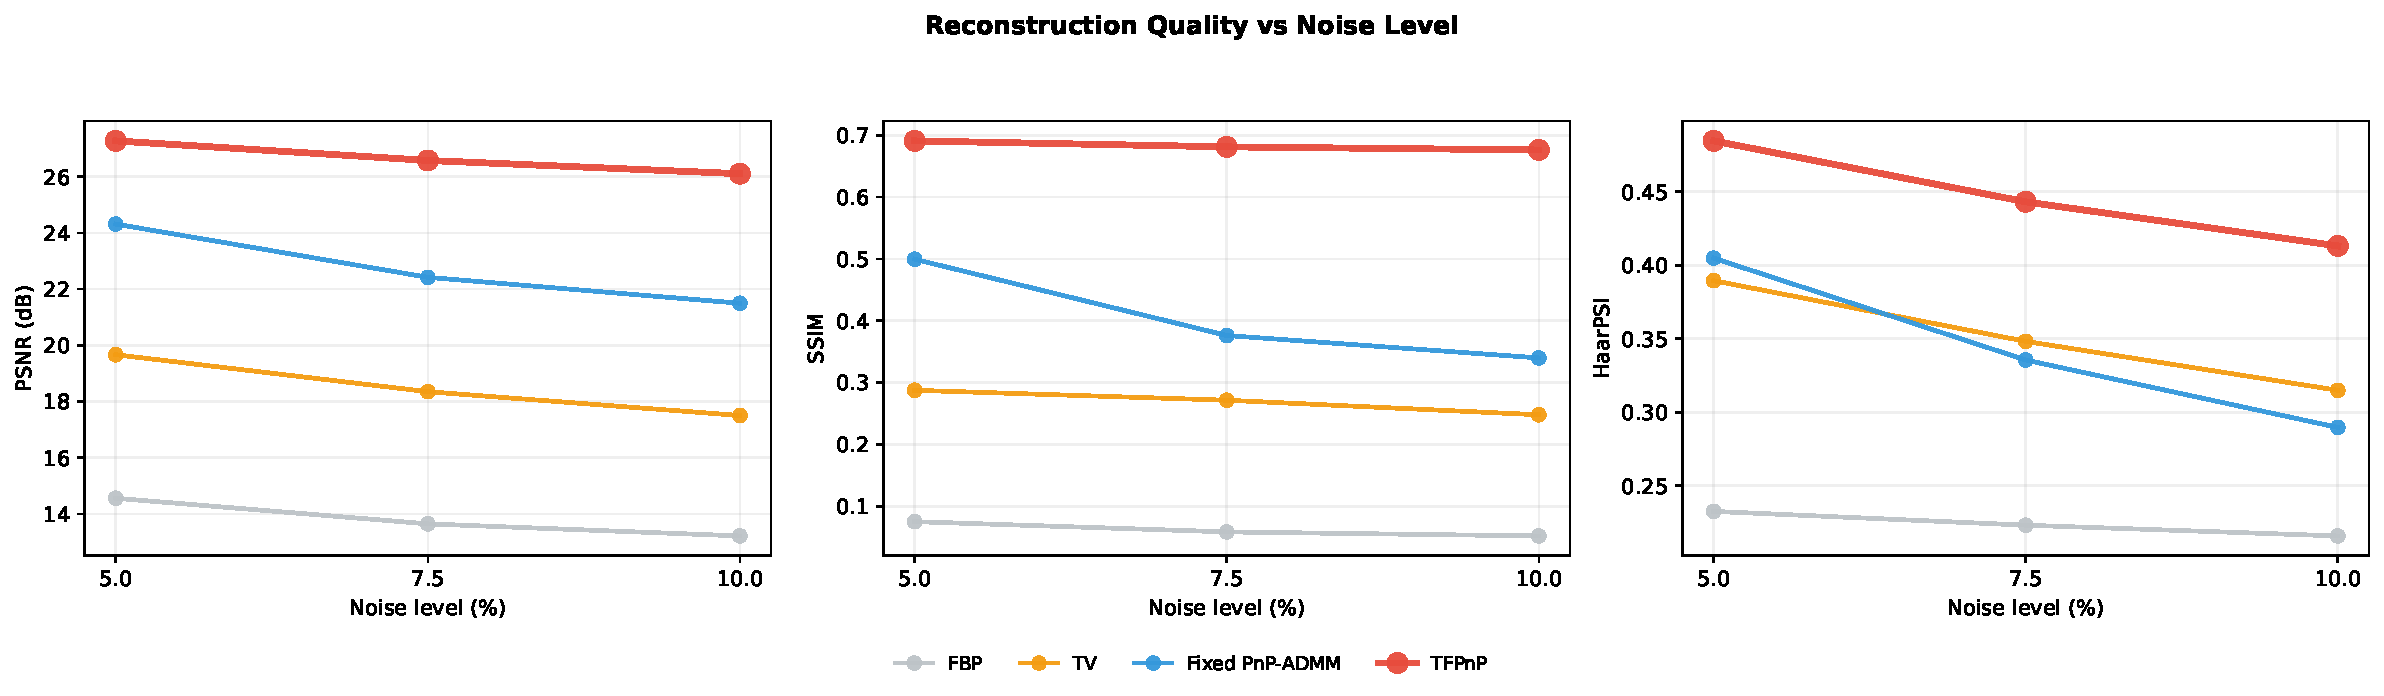
\includegraphics[width=\linewidth]{../figures/run_04_pat_250_e80/metrics_vs_noise.pdf}
    \caption{Mean PSNR, SSIM, and HaarPSI vs sinogram noise level.}
    \label{fig:metrics_vs_noise}
\end{figure}

\textbf{CT-specific denoiser extension.} A CT-DRUNet was trained on LIDC to test whether an in-domain denoiser would improve reconstruction. In the Fixed PnP-ADMM setting, it outperforms the natural-image DRUNet at every noise level, with the advantage growing under noise ($+0.71$\,dB at 5\% to $+1.98$\,dB at 10\%). Because each denoiser is compared at its own calibrated optimum, this improvement directly relates to in-domain training, and stands independently of the full RL pipeline.

\textbf{Reward-shaping ablation.} A second extension tested if alternative reward signals (SSIM, HaarPSI, and mixed PSNR-perceptual rewards) would improve metric-specific performance, motivated by evidence~\citep{breger2025study} that PSNR correlates poorly with perceived quality, especially in medical imaging. Across four trained variants, the SSIM-only reward achieved the highest PSNR and HaarPSI, the mixed PSNR/SSIM reward won on SSIM, and both HaarPSI rewards underperformed. This inconsistency helped establish PSNR on its own as a defensible reward signal for this reproduction.

\textbf{Corrections and planned work.} All experiments ran on the CSD3 cluster under a single GPU account, which capped the number of ablations, and three of the paper's six baselines (RED-CNN, LPD, RPGD) could not be added as they are either absent from LION or training would exceed the timeline of the project. Retraining the TFPnP policy against the CT-DRUNet initially failed, with the critic loss diverging and the policy $\sigma$ output collapsing, but diagnosis traced this largely to a calibration artefact in the training script. Relevant corrections were made but could not be run due to the cluster outage so remain as future work. This is also the case for a prepared FBPConvNet extension, which trains the baseline on a mixed nosie regime to better match the implementation.

\textbf{Contributions and lessons.} The project contributes a tested TFPnP reproduction that confirms the paper's central claim of TFPnP producing better results compared to hand-tuned PnP-ADMM, as well as the finding that in-domain FBPConvNet training reverses the paper's ranking at low noise while TFPnP has an advantage at high noise. A CT-DRUNet extension improving Fixed PnP-ADMM by $+0.71$--$+1.98$\,dB suggested that in-domain training has significant benefits for the reconstruction quality, and a reward-shaping ablation confirmed the PSNR reward as the correct default. A pull request (\#184) to the LION toolbox with corrections to the FBPConvNet implementation was also carried out as part of this project. The two main conclusions are that evaluating every learned method out-of-domain, as the paper does for fairness, can under-represent methods on a specific medical domain, so PnP methods should be compared against domain-adapted baselines whenever possible, and TFPnP's tuning-free claim holds at inference but not during development, where action ranges, learning rates, and reward functions all require careful choices, making the method tuning-free to use, not tuning-free to build.

\bibliographystyle{plainnat}
\bibliography{bibliography}

\end{document}